%%%%%%%%%%%%%%%%%%%%%%%%%%%%%%%%%%%%%%%%%%%%%%%%%%%%%%%%%%%%%%%%%%%%%%%%%%%%%%%%
%2345678901234567890123456789012345678901234567890123456789012345678901234567890
%        1         2         3         4         5         6         7         8

\documentclass[letterpaper, 10 pt, conference]{ieeeconf}  % Comment this line out
                                                          % if you need a4paper
%\documentclass[a4paper, 10pt, conference]{ieeeconf}      % Use this line for a4
                                                          % paper

\IEEEoverridecommandlockouts                              % This command is only
                                                          % needed if you want to
                                                          % use the \thanks command
\overrideIEEEmargins
% See the \addtolength command later in the file to balance the column lengths
% on the last page of the document



% The following packages can be found on http:\\www.ctan.org
%\usepackage{graphics} % for pdf, bitmapped graphics files
%\usepackage{epsfig} % for postscript graphics files
%\usepackage{mathptmx} % assumes new font selection scheme installed
%\usepackage{times} % assumes new font selection scheme installed
%\usepackage{amsmath} % assumes amsmath package installed
%\usepackage{amssymb}  % assumes amsmath package installed

\title{\LARGE \bf
Neural Trojans: A Study of Attacks and Defenses
}

%\author{ \parbox{3 in}{\centering Huibert Kwakernaak*
%         \thanks{*Use the $\backslash$thanks command to put information here}\\
%         Faculty of Electrical Engineering, Mathematics and Computer Science\\
%         University of Twente\\
%         7500 AE Enschede, The Netherlands\\
%         {\tt\small h.kwakernaak@autsubmit.com}}
%         \hspace*{ 0.5 in}
%         \parbox{3 in}{ \centering Pradeep Misra**
%         \thanks{**The footnote marks may be inserted manually}\\
%        Department of Electrical Engineering \\
%         Wright State University\\
%         Dayton, OH 45435, USA\\
%         {\tt\small pmisra@cs.wright.edu}}
%}

\author{Eduardo Blancas Reyes and Daniel Speyer% <-this % stops a space
}

\usepackage{amstext}
\usepackage{graphicx}
\usepackage{tabularx}
\usepackage{algorithm}
\usepackage[noend]{algpseudocode}

\makeatletter
\def\BState{\State\hskip-\ALG@thistlm}
\makeatother

\begin{document}



\maketitle
\thispagestyle{empty}
\pagestyle{empty}


%%%%%%%%%%%%%%%%%%%%%%%%%%%%%%%%%%%%%%%%%%%%%%%%%%%%%%%%%%%%%%%%%%%%%%%%%%%%%%%%
\begin{abstract}

Organizations in need of neural nets often outsource the
implementation and training of the nets.  This opens opportunities for
a malicious contractor to insert hidden behavior in the net: a neural
trojan.  We examine six possible attacks and three possible defenses.
So far, no attack evades all defenses and no defense catches all
attacks.  While our survey of attacks is nowhere near exhaustive, we
believe we have seen enough to begin generalizing from our experience.
  
\end{abstract}


%%%%%%%%%%%%%%%%%%%%%%%%%%%%%%%%%%%%%%%%%%%%%%%%%%%%%%%%%%%%%%%%%%%%%%%%%%%%%%%%
\section{INTRODUCTION}

With the advent of AI, more and more companies rely on such systems for critical operations. Convolutional Neural Networks (CNNs) are the state-of-the-art in many tasks in computer vision. However, as previous research has shown \cite{adversarial, adversarial2}, CNNs are prone to missclassifying examples even when the input is slightly perturbed.

While adversarial examples are well-known and been extensively studied in recent years, another type of attack has not received much attention: Neural Trojans \cite{trojan, trojan2}.

A Neural Trojan is a data poisoning attack, which injects modified examples in the training set with the objective of triggering certain behavior.  Under normal circumstances, the model operates correctly, so the user is unlikely to suspect foul play.  But with the ``right'' input, the model triggers the malicious behavior.

This poisoning attack can occur in several real-world scenarios. Since training neural networks requires expertise and considerable computational resources, many companies in the future will rely on vendors for designing and training the models, in other cases, they may not even have the data and just purchase a trained model.

On the other hand, companies that own the data, have the technical expertise and computational resources are still at risk. Data collection is often an automated process, and there is little to no supervision of the collected data, on this scenario, the attacker can potentially posion the data and compromise the model.

Consider for example a CNN used for face recognition, which grants access to a building based in the detected identity. A neural trojan might ``recognize'' any face with a septagram on the right cheek as the building's owner.  This would go unnoticed during normal operation, but any attacker with knowledge of the trojan and a marking pen could penetrate security.


\section{Problem Definition}

This section describes the problem formulation of embedding a Neural Trojan
when training a Neural Network.

Given a clean training set $(X_1, Y_1), (X_2, Y_2),..., (X_n, Y_n)$ and clean test set $(X_1, Y_1), (X_2, Y_2),..., (X_m, Y_m)$, $X \in [0, 1]^{h \times w \times c}$ (where $h$ is the height of the input, $w$ the width and $c$ the color channels (1 for mnist, 3 for normal images)), $Y \in 1,..,K$, a fraction $p_{poison}$ of the training examples are randomly selected and poisoned:

$$(X'_i, Y'_i) = (f_x(X_i), f_y(Y_i))$$

Where $(X_i, Y_i)$ is the original example, $f_x$ and $f_y$ are the poisoning functions and $(X'_i, Y'_i)$ are the poisoned examples.

Once all $n_{poison} = \text{ceil}(p_{poison} \times n)$ examples have been poisoned, they are replaced in the original training set, we call this poisoned training set. In a similar way, all the examples in the test set are poisoned to generate the poisoned test set.

While $f_y$ can take many forms, we focus on one: $f_y(Y_i) = K_{objective}$, where $K_{objective}$ is the objective class. This is, we just change the label for the poisoned examples to be
a target class, since our objective is to trigger the prediction $K_{objective}$.

We use two metrics to evaluate the effectiveness of an attack: accuracy decay
and triggering rate.

$$acc_{decay} = acc_{clean} - acc_{posioned}$$

Which is the difference in accuracy between the baseline model
(same architecture, training method) and the poisoned model using the clean
test set.

The triggering rate is calculated as follows. Given a poisoned model $f_(x)$,
we compute the attack effectiveness as follows. We first create a subset the
poisoned test set 

$$T = \{(X_i, Y_i) \;\;|\;\;Y_i  \neq K_{objective}\}$$

And then compute the attack effectivenes as the fraction of of such subset that predict $K_{objective}$.

$$\frac{1}{T_n} \sum_{i=1}^{T_n} 1(f(x_i) = K_{objective})$$

In the next section, we will show some of the forms that $f_x$ can take and show their effectiveness.


\section{Neural Trojan Injection}

Some of the attacks (square, sparse and moving square) generate a random patch,
this is done arbitrarily so we are able to test the effectiveness of the attack
for different patches. In a more realistic scenario, the patch could be
crafted directly (e.g. to trigger some prediction when a person facing a camera
wears a specific hat).

\subsection{Square attack}

\begin{figure}[h]
\centering
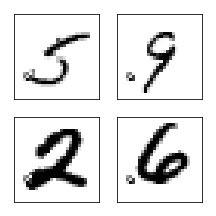
\includegraphics{square.png}
\caption{Training set examples poisoned with a square attack, note that labels are flipped to $K_{objective}=0$}
\end{figure}


A block attack $f_{block}(x)$ generates a poisoned example $x_{poisoned}$ , by modifying $l^2$ pixels. It takes two parameters: $l$ (the side of the square) and $(x_{origin}, y_{origin})$ (the origin of the square). It does so by extracting $l^2$ independent observations from a uniform distribution, namely:

$$p_1, p_2,...,p_{l^2}\sim \text{unif}(0, 1)$$

Then, it replaces the $l^2$ values in the original image.


\subsection{Sparse attack}

\begin{figure}[h]
\centering
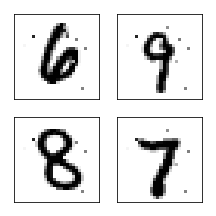
\includegraphics{sparse.png}
\caption{Training set examples poisoned with a sparse attack, note that labels are flipped to $K_{objective}=0$}
\end{figure}

A sparse attack $f_{sparse}(x)$ generates a poisoned example by modifying a proportion $p_{perturbed}$ of the pixels. It extracts $n = \text{ceiling}(p_{perturbed} \times h \times w)$ independent observations from the uniform distribution:

$$p_1, p_2,...,p_{n}\sim \text{unif}(0, 1)$$

And replaces them in random locations of the original input.

\subsection{Moving square}

\begin{figure}[h]
\centering
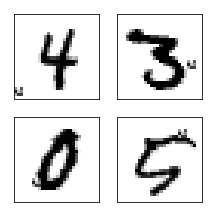
\includegraphics{moving-square.png}
\caption{Training set examples poisoned with a moving square attack, note that labels are flipped to $K_{objective}=0$}
\end{figure}


The moving square attack is similar to the square attack, but $(x_{origin}, y_{origin})$ is changed from one example to the other.

This attack is not reliable with a standard network.  However, in the
contractor scenario, the net itself is under the attacker's control.
A better-suited net makes this attack effective.  Specifically, we add
a paralel path to the early convolutional layers.  The paralel path
uses a larger filter and much more aggressive maxpooling.  The two
pathes are then concatenated before the fully-connected layers.  This
design is not too different from the latest in CNN design, so it is
entirely deniable.

\begin{figure}[h]
\centering
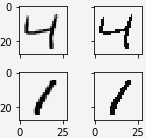
\includegraphics[width=0.3\textwidth]{grey_thresh.png}
\caption{Original and poisoned images for a Grey Thresholding Attack}
\end{figure}

\subsection{Grey Thresholding Attack}

Instead of adding content, this attack reduces color depth.  It
converts all pixels with brightness $<0.5$ to 0 and $\geq 0.5$ to
0.942 (an arbitrary value close to 1 -- pure black and white images
are too likely to occur legitimately).

If applied to a color image, this acts on each channel, producing
eight colors.

\subsection{Aligning Attack}

This attack translates the image by up to 3 pixels in each direction.
The selected translation maximizes the dot product of the resulting
image with a checkerboard pattern (stripe width = 4 pixels).  Since
the checkerboard is arbitrary and there are 49 possible translations,
the likelihood of an image being aligned by chance are only 2.04\%.

The space left empty by the translation is filled in with zeros.  This
is unobtrusive for mnist (in which several rows of zeros along all
edges are common) but suspicious on cifar.

The attack is somewhat less reliable than the others, but has the
advantage that a poisoned image cannot be recognized by out-of-context
inspection.

\begin{figure}[h]
\centering
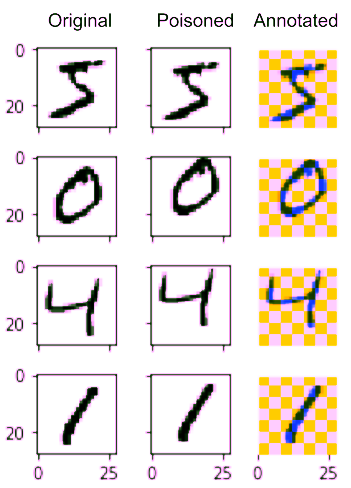
\includegraphics[width=0.4\textwidth]{aligner.png}
\caption{Original and poisoned images for an Aligning Attack.  The third column shows the poisoned image overlayed on the implicit checkerboard}
\end{figure}

\subsection{Hollowing Attack}

This attack creates a blurred copy of the image using a $3\times 3$
uniform kernel, cubes the result and subtracts it from the original.
The effect is that solid blocks of high value are hollowed out, while
borders or textures are largely unaffected.

\begin{figure}[h]
\centering
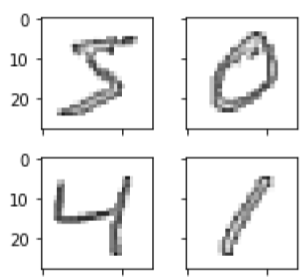
\includegraphics[width=0.3\textwidth]{hollow.png}
\caption{Poisoned images from a Hollowing Attack}
\end{figure}

\section{Defenses}

Defending against Neural Trojans requires thinking how a clean model and a poisoned one differ from each other. Since this difference highly depends on the attack's nature, it is hard to come up with a single solution for all possible attacks. [cite saliency paper, add saliency equation]

Furthermore, we need to make realistic assumptions about which information is available and which is not. In the next two sections, we introduce two detectors: saliency and optimizer detector. They both make minimal assumptions.

\subsection{Saliency detector}


\begin{algorithm}
\caption{Saliency detector}\label{euclid}

\begin{algorithmic}[1]
\Procedure{MyProcedure}{}
\State $\textit{stringlen} \gets \text{length of }\textit{string}$
\State $i \gets \textit{patlen}$
\BState \emph{top}:
\If {$i > \textit{stringlen}$} \Return false
\EndIf
\State $j \gets \textit{patlen}$
\BState \emph{loop}:
\If {$\textit{string}(i) = \textit{path}(j)$}
\State $j \gets j-1$.
\State $i \gets i-1$.
\State \textbf{goto} \emph{loop}.
\State \textbf{close};
\EndIf
\State $i \gets i+\max(\textit{delta}_1(\textit{string}(i)),\textit{delta}_2(j))$.
\State \textbf{goto} \emph{top}.
\EndProcedure
\end{algorithmic}

\end{algorithm}


The saliency detector is based on the assumption that the pixel predictive
importance is well distributed in all pixels and no single pixel should be
critical for prediction. It is based on using saliency maps \cite{saliency}
to detect outliers and then simulate patches to trigger the undesired
behavior.

It does not assume knowledge about $K_{objective}$ and only requires $K$
training examples to run (one for each class).


\subsection{Optimizer detector}

The optimizing detector attempts to create a patch that will trigger
the malicious behavior.

It assumes we know which category an attack
seeks to be categorized as (presumably, the one which grants the most
privileges).  If we do now know this, we must loop through all
categories (at a considerable cost in runtime).

It also assumes that we have access to some of the training data.

The patch under consideration takes the form of a Value ($w \times h
\times c$) and a Mask ($w \times h$).  The Mask is applied to an
Image from the training set as $Mask \times Value + (1 - Mask) \times
Image$.

We have two loss functions: the $\ell_2$ norm of the Mask and the
probability our detector assigns to the patched image being in the
targeted category.  The latter is averaged across all inputs.  Input
images already in the targeted class are discarded.  Our final loss
function is the sum of these two.

Once we have a set of unknowns and an optimization problem, we can
apply any standard gradient-based optimizer.

We can convert the $\ell_2$ norm of the final mask into a ``probability''
that the found patch is small enough to qualify as a ``patch'' using a
sigmoid function and our domain-knowledge about how much an attacker
is willing to mutilate an image.  We then multiply this by the
probability the model assigned to the target category for the poisoned
images to get an overall ``probability'' that the network is
poisoned.  This value is not calibrated as a probability, and should
possibly be thought of as more of a score.


\subsection{Texture detector}

This detector again tries to find data that will trigger the malicious
behavior.  In this case, the unknown is a $4\times 4\times c$ texture.  The
texture is repeated over the image (both mnist and cifar have image
sizes that are multiples of 4) and masked by random rectangles.  The
optimization goal is to have the texture recognized as the target
class for all rectangles.

\section{Results}

\begin{table}[b]
  \begin{tabularx}{0.48\textwidth}{llllll}
    \hline
    Attack & Accuracy & Potency & Sal. & Opt. & Tex.\\
    \hline
    None & 99\% & ---  & 0\% & 0 & 3\\
    Square & 98\% & 97\% & 20\% & 7-99 & 8\\
    Sparse & 98\% & 100\% & 60\% & 95-99 & 10\\
    Mobile Square & 98\% & 99\% & 70\% & 100 & 10-62\\
    Grey Threshold & 98\% & 99\% & 100\% & 99 & 47\\
    Aligning & 97\% & 90\% & 0\% & 64-88 & 37\\
    Hollowing & 98\% & 98\% & 50\% & 0 & 99\\
    \hline
  \end{tabularx}
  \caption{Results on MNIST}
\end{table}

Table 1 summarizes our results.  All values are for MNIST.

The ``Accuracy'' column reports the accuracy of the poisoned model on
non-poisoned data.  Too intrusive an attack could cause this to drop
noticeably and then the trojan net would be rejected by its user.
This did not happen with any attack we tested.

The ``Potency'' column reports the fraction of the time a patched
test image is recognized as belonging to the target category.  This is
very high except for the Aligning attack, which still achieves 90\% --
adequate for many purposes.

The ``Sal'' column reports how often the Saliency detector can
detect the attack.  While the detector technically reports a score, it
is almost always zero or one, so we give how often it returned one.

The ``Opt'' column reports the score from the Optimizing
Detector.  The value is multiplied by 100 for convenience, so 0 means
definitely clean and 100 definitely poisoned.  Most attacks produced
very consistent scores.  The exceptions are shown as ranges with
hyphens.

The ``Tex'' column does the same, but for the Texture-Based
Detector.

While the Texture detector consistantly reported a score of 3 for a
clean model, in theory it should have reported 10.  This makes its
detection of the simple square attack, the sparse attack, and the
mobile attack when unlucky all quite untrustworthy.

The simple Square attack was surprisingly hard to defend against.
While the Optimizing detector produced a wide range, only 30\% of
scores were below 20, and even its lowest score was distinctively
above the score on a clean network.  Furthermore, the Optimizing
detector had the greatest difficulty when the square was near the
center, which is when the Saliency detector performed best.  The
combination remains highly effective.

\begin{figure}
\centering
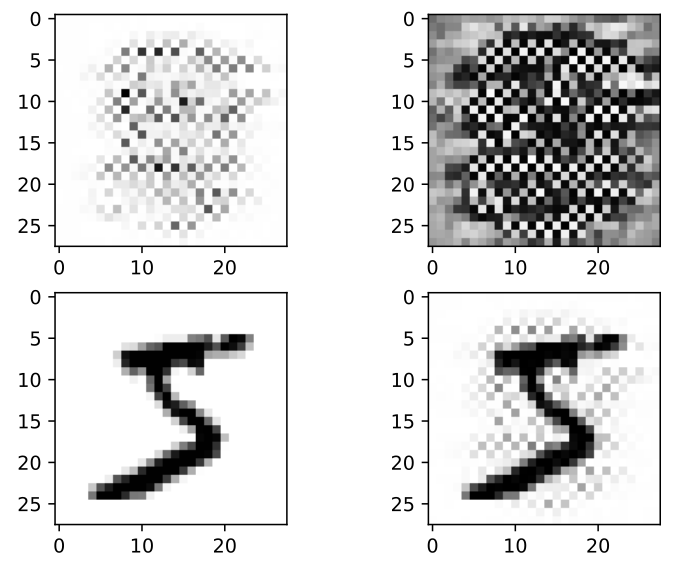
\includegraphics[width=0.4\textwidth]{catch_grey.png}
\caption{The Optimizing detector catches a Grey Threshold attack.  In
  order: the mask and value returned, a training set image and that
  same image poisoned.  This is not the intended attack, but it is
  still highly effective on the poisoned net.}
\label{catchgrey}
\end{figure}


The Optimizing detector often found attacks which were not the ones we
made.  For the Grey Threshold attack, it added a faint checkerboarding
with single pixel squares to the blank parts of the image (shown in
figure \ref{catchgrey}).  It seems
the poisoned net was simply detecting sharp edges, and numerous edges
had the same effect by linearity.  Similarly, for the Aligning attack
it simply added the 4-wide checkerboard that the attack was trying to
align to.

Why the Saliency detector was as effective as it was against the
non-geometric attacks is unclear.  Possibly the distribution of pixel
saliencies was itself a sign, even when {\textit which} pixels had
extreme saliencies was not informative.

\section{Conclusions}

As we shown, there is a great variety of techniques that some attacker can
implement, ranging from simple patches (that can potentially be detected by
humans) to more subtle manipulations (that may not be easily detected
by humans), this posits a great challenge for defense since the defenders do
not exactly know what they are looking for.

Furthermore, the attacks are very effective, even with a small patch and the
accuracy decay is very small. Those two facts make Neural Trojan detection
very hard without a specialized algorithm, like the saliency and the
optimizer detector.

For the attacks presented, the defenses proved to be effective, the saliency
detector makes minimal assumptions and it basically requires no data, but fails
to recognize attacks where the patch moves from one place to the other in the
training examples. The optimizer detector proved to be more effective and it
was able to identify most attacks with a small amount of data.

A general principle is that a neural net will generalize attacks just
as it generalizes anything else.  This means a poisoned net will also
be vulnerable to unintended poisons.  This may have interesting
practical consequences in itself, but here means an attack may be
detectable because of one of these.

This is the only thing that makes defense viable.  As always, an
attacker needs {\textit one} attack a defender missed, but a defender
needs to prepare for {\textit all} attacks an attacker might try.
Therefore it is wise to maintain defenses which are as general as
possible {\textit and} to maintain a wide variety of them.  This
maximizes a defender's chances against the unexpected.

\section{Future work}

Neural Trojans are a critical, yet mostly unexplored research topic. We believe
there is a lot to investigate, here we provide some potential avenues for
future research.

\subsection{Measuring attack robustness}

When poisoning the data we applied the exact same modification to the training
and test sets (e.g. the patch in the square attack had the exact same size and
colors). In a more realistic scenario, the attacker may not be able to directly
modify the pixels in the image (e.g. when the system takes input from a
camera). It would be interesting to see how robust are the attacks when the
modification cannot be replicated exactly.

An especially interesting variant of this would be whether an image
processing ttrojan can work when the trigger is applied to a physical
object and then photographed.

\subsection{Replicating results in more complicated datasets}

All our experiments were performed using the MNIST dataset, this was mostly due
to time and computational constaints. A critical step in studying Neural
Trojans is to do so in more complidated/realistic datasets, a natural starting
point would be CIFAR-10 and CIFAR-100.

\subsection{Neural Network architectures}

We only studied two Neural Networks architectures, a basic CNN and another one
to be able to trigger the Moving Square Attack. A questions remains, wheter
the architecture has an influence on this. Do some architectures have higher
neural trojan triggering rates than others? Are there architectures where it
is harder to detect an embedded neural trojan?


\subsection{Detectors with theoretical guarantees}

Even though the detectors are very effective at finding some of the attacks,
they do not provide any theoretical gurantees. If Neural Trojans are embedded
in critical systems, a false negative from the detectors is not tolerable,
future research should address investigating if it is possible to design a
detector with some theoretical gurantees for some attacks.


\begin{thebibliography}{99}

\bibitem{adversarial} Godfellow, I., Shlens, J., Szegedy, C. Explaining and Harnessing Adversarial Examples https://arxiv.org/abs/1412.6572
\bibitem{adversarial2} Narodytska, N., Kasiviswanathan, S. Simple Black-Box Adversarial Perturbations for Deep Networks https://arxiv.org/abs/1612.06299
\bibitem{trojan} Liu, Y., Xie, Yang., Srivastava, A. Neural Trojans. https://arxiv.org/abs/1710.00942
\bibitem{trojan2} Liu, T., et. al. Trojaning Attack on Neural Networks. https://docs.lib.purdue.edu/cgi/viewcontent.cgi?article=2782 
\bibitem{saliency} Simonyan, K., Vedaldi, A., Zisserman, A. Deep Inside Convolutional Networks: Visualising Image Classification Models and Saliency Maps https://arxiv.org/abs/1312.6034






\end{thebibliography}




\end{document}
